\subsection{Сформулировать, какие частицы называются бозонами, привести примеры Бозе-частиц.
Сформулировать правило заполнения состояний Бозе- частицами. Используя формулу Больцмана
для энтропии, вывести распределение Бозе-Эйнштейна}

Вывод аналогичен выводу распределения Ферми-Дирака, см. \ref{fermi-dirak}.

Рассмотрим область, разделенную на $Z$ ячеек с помощью $Z-1$ перегородок.
\begin{figure}[H]
	\centering
	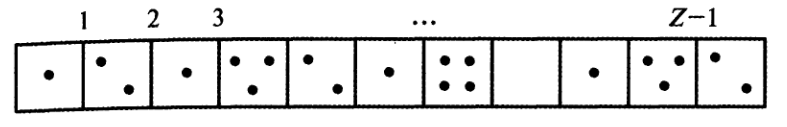
\includegraphics[width=0.7\linewidth]{img/write-06/yacheiki}
	\caption{Возможное распределение бозе-частиц по ячейкам}
	\label{fig:yacheiki1}
\end{figure}

% Система состоит из $N$ частиц, $Z-1$ перегородок, $N+Z-1$ элементов всего. Посчитаем статистический вес.

% Идет речь о перестановке не только частиц с частицами, но и перегородок с перегородками. Могут переставляться и частицы вместе с перегородками. Общее число $(N+Z-1)!$. Учтем перестановки частиц (т.к. они неразличимы), поделим на $N!$. Учтем перестановки неразличимых перегородок, поделим на $(Z-1)!$.
Число способов $\Omega$, с помощью которых $N$ тождественных частиц могут быть
распределены по $Z$ ячейкам равно
\begin{equation*}
  \Omega = C^N_{N+Z -1} = \frac{(N+Z-1)!}{N!(Z-1)!}.
\end{equation*}

Далее все аналогично выводу распределения Ферми-Дирака (см. выше).
После применения метода неопределенных множителей Лагранжа:
\begin{equation*}
	\frac{N_i+Z_i-1}{N_i} = \exp \left\{-\frac{\lambda_2E_i-\lambda_1}{k}\right\}
\end{equation*}
И так далее аналогично.

\begin{equation*}
  \langle n\rangle_\textsc{Б-Э} = \frac{1}{\exp\left\{\frac{E-\mu}{kT}\right\}-1}
\end{equation*}

\begin{figure}[H]
	\centering
	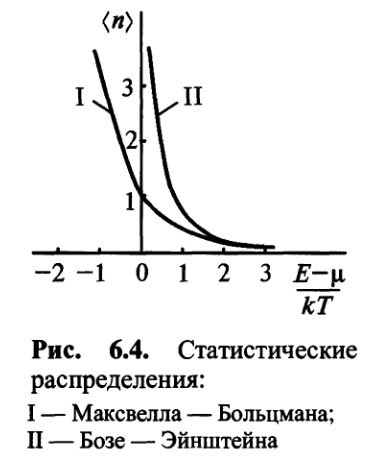
\includegraphics[width=0.4\linewidth]{img/write-06/bose-einstein}
%	\caption{}
	\label{fig:bose-einstein}
\end{figure}
